\chapter{Background}

\textbf{TODO introduce chapter}

\textbf{lorem ipsum}

\textbf{Maybe mention transparencies somewhere}

\section{HTLM and the DOM}

Web pages are composed of \ac{HTML} and \ac{CSS} documents. \ac{HTML} and \ac{CSS} are declarative programming languages that define the content and styling of web pages \cite{Lie1999}. This means that the \ac{GUI} of a web page is defined by the content of the corresponding \ac{HTML} and \ac{CSS} documents. As \ac{HTML} and \ac{CSS} can be seen as being complementary technologies, and is often used together, all uses of \ac{HTML} will be a reference to both \ac{HTML} and \ac{CSS} for the rest of the thesis. \ac{HTML} was both meant to be written by humans, and generated by computer applications (front-end applications) \cite{Lie1999}. The process of when a front-end application generates \ac{HTML} documents is called rendering.

Front-end applications can be categorized into 5 categories, which are presented in Figure \ref{fig:fe-render-methods}. They are categorized on when, and how close to the client device, the rendering process is executed. Static \ac{HTML} is when a developer manually writes \ac{HTML}. Pre-rendering is when a developer uses another markup language than \ac{HTML}, and then uses a tool to render the markup into \ac{HTML}. The server in this case, where the render is performed, does not necessarily have to be the same server that serves the \ac{HTML} to clients. It is used to describe a computer that is not the client. Pre-rendering is done either for a simpler development process, or for use cases that require a larger feature set than static \ac{HTML} can provide. Server Side and Client Side Rendering is when \ac{HTML} is rendered in run time, which is often done for dynamic content or interactive behaviour. Different rendering methods can be mixed for different parts of a web page. If both server side and client side rendering is used for the same parts, it is called Isomorphic rendering.

\begin{figure}
    \centering
    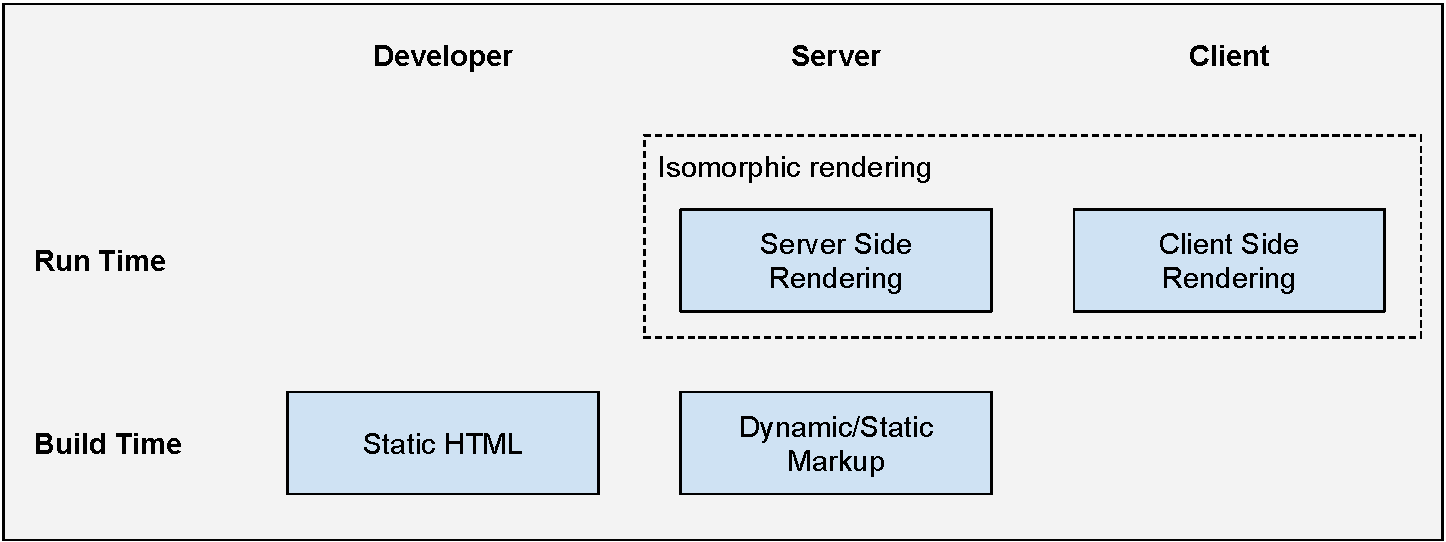
\includegraphics[width=\linewidth]{images/fe-rendering.pdf}
    \caption{Different methods for generating \ac{HTML}. When it is done by a server or client device it is called rendering. Multiple methods can be used for the same web page, and if it is done using different methods, for the same part of the page, it is called isomorphic rendering.}
    \label{fig:fe-render-methods}
\end{figure}

\subsection{Pre-rendering and Server Side Rendering}

Pre-rendering static markup is when tools are used that transform files from one markup format into \ac{HTML}. This is often done in build-time. Pandoc is a tool that translates simpler markdown formats to \ac{HTML} \cite{Dominici2014}. The most prominent benefit is that more lightweight markup languages can be quicker and easier to use when developing web pages as they are more human readable and less verbose, at the cost providing a more limited feature set \cite{Dominici2014}.

There also exists markup languages like PHP that provide a larger feature set than \ac{HTML}. These can provide imperative programming constructs that allow access to perform network calls, composition of reusable components, or resolve database queries \cite{Royappa2000}. These front-end applications can execute their render both in build-time or run-time, depending on if they have to provide dynamic content based on the client request. Dynamic refers to the dynamic nature of the content, where the content is mutable, persistent or user customized. If the render is executed in build time it is pre-rendering based on dynamic content, and if it is done in run time it is called server side rendering.

\subsection{Client Side Rendering}

A front-end application can also be client based where a client receives one or many scripts, that manipulate the \ac{HTML} document. This results in \textit{interactive} applications where user interactions result in animations or GUI changes, without a page refresh. To facilitate this, browsers expose an API, called \ac{DOM}, that allows scripting languages to access and manipulate \ac{HTML} documents \cite{Apparao1998}. This is most commonly done using JavaScript. Already in the beginning of the 2000's researchers experimented with client side rendering, where JavaScript was used to update the \ac{GUI} without a page refresh \cite{Betz2000}.

\textbf{AJAX and asynchronous updates.}

Client side rendering can also be used to render all of the content of a web page, and even simulate page navigation by re-rendering most or all of the web page. This type of front-end application is called \ac{SPA}, because of how the full front-end application is included in one page \cite{Mesbah2007}. Sometimes the different navigation methods are called hard and soft navigation, where soft navigation is when the navigation is simulated by a client side front-end application.

All different front-end applications methods can be mixed where different parts of the \ac{HTML} document is rendered using different methods. If the same parts are rendered both by the server and the client, it is called \textit{isomorphic rendering} \cite{Brehm2013} or universal application \cite{alabes2017isomorphic}. The concept is that a web page is first rendered at the server, sent in a rendered state to the client, and then a replica of the front-end application is sent to the client. When the replica has been loaded on the client, the web page is re-rendered and acts as a traditional \ac{SPA}. The benefit compared to a traditional \ac{SPA} is that the web page is loaded quicker, as the initial file contains all required \ac{HTML} to show the web page \cite{Brehm2013}. It also improves search engine performance, and allows users to optionally use JavaScript\cite{Brehm2013}.

\section{Modern web development}
\subsection{Patterns}
\textbf{discuss modern web applications. Props down, events up. One way data flow}
\subsection{Tools}
\textbf{react/vue, webpack/babel, node, npm/package.json, typescript}

\section{Component Composition}

\textbf{Write about all kinds of approaches to compose a gui of multiple components. Preferably in run time.}

\textbf{Portlets and Mashlets (web mashups)}

\textbf{Transclusion}

\section{Microservices (this section will be re-written)}

\textbf{Focus more on what microsercvices are. The definition.}

Microservices is a software development method where systems are divided into smaller parts, called microservices, that can be individually deployed \cite{Newman2015a}. In turn, this enables low coupling, high cohesion, and strong composability \cite[ch.~1]{Newman2015a}. It also enables multiple developers to work on a shared codebase while minimizing obstruction, which becomes more notable in larger systems, with a large number of developers \cite{Newman2015a}. This concept is also referred to as team independence.

% Microservices are focused on performing single tasks really well, and implementing functionality by composing multiple microservices.

A central aspect of microservices is the concept of ``vertical slicing'' as a decomposition strategy, which is an important facilitator of team independence \cite{Familiar2015}. An example of vertical slicing can be seen in Figure \ref{fig:vertical-slicing}. An early adopter of vertical slicing was \citeauthor{Ratner2011} who observed agile teams who broke up user stories into multiple horizontal layers. They observed that teams focused on one part of the technology stack at a time, which resulted in stories that provided non user facing changes. Vertical slicing solves this by defining stories and responsibilities that encompass end-to-end functionality. This means that instead of thinking in terms of user interface, business logic, and data storage as separate distinct horizontal layers, a story should include all of them, but only from a narrow context \cite{Ratner2011}. \citeauthor{Ratner2011} describes their method as \blockquote{[...] driving a thin vertical slice from UI to database, which is functionally coherent and demonstrable, then progressively widening it with consecutive slices. \cite{Ratner2011}}

\begin{figure}
    \centering
    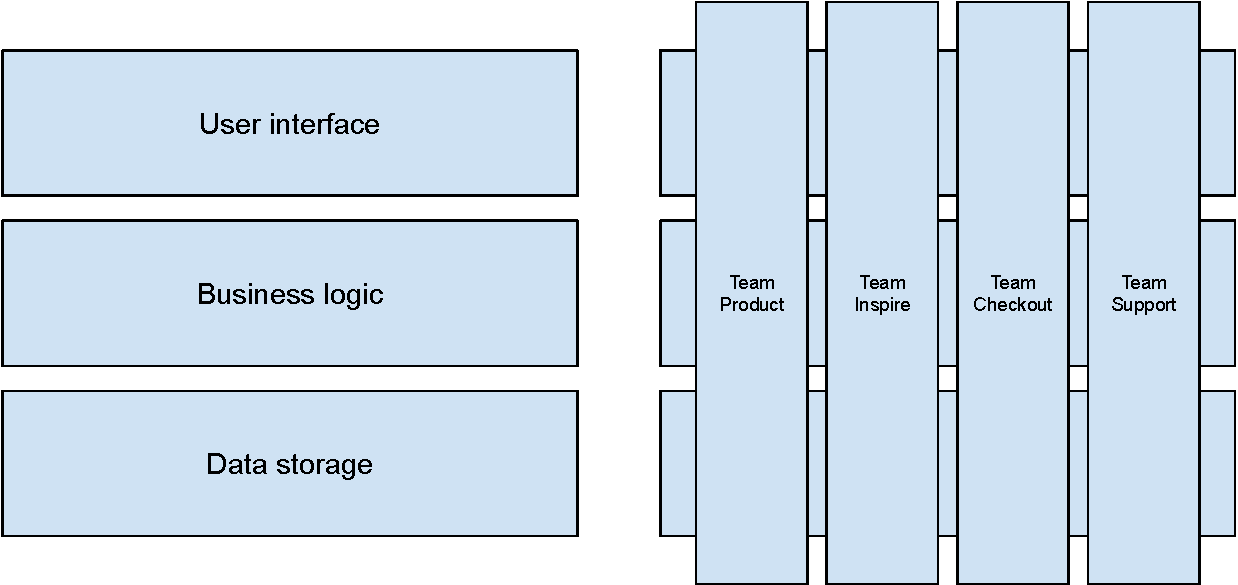
\includegraphics[width=\linewidth]{images/vertical-slicing.pdf}
    \caption{Horizontal Layering and Vertical Slicing. This is an example of four cross functional development teams that are responsible for all aspects of delivering a customer facing feature.}
    \label{fig:vertical-slicing}
\end{figure}

Vertical slicing can be applied to stories like \citeauthor{Ratner2011} describe \cite{Ratner2011}, to team responsibilities, and to system design \cite{Geers2020}. Vertical slicing is a consequence of cross functional agile teams \cite{Geers2020}, which can be explained by Conway's law: \blockquote{Any organization that designs a system (defined broadly) will produce a design whose structure is a copy of the organization's communication structure \cite{Conway}.} This can be interpreted as vertical slicing of system components being a consequence of smaller cross functional teams.

\section{Semantic Versioning and Lock-step Deployments}

See page 64-65 in ``Building Microservices (Sam Newman)''

Gradual Migration

\section{Vertical Decomposition and Self-Contained Systems}